\chapter{电磁学}

\newpage
{\bf 这里是一段关于电磁学的介绍.}

\newcommand\resistance{
	\begin{tikzpicture}[baseline = {([yshift = -3.5pt] current bounding box.center)}]
		\draw (0, 0) rectangle (0.6, 0.2);
		\draw (-0.3, 0.1) -- (0, 0.1);
		\draw (0.6, 0.1) -- (0.9, 0.1);
	\end{tikzpicture}
}

\newcommand\ammeter{
	
\begin{tikzpicture}[baseline = {([yshift = -3.5pt] current bounding box.center)}]
		\node (A) [circle, draw, scale = 1, inner sep = 1pt, line width = 0.5pt] at (0, 1){\small A};
	\end{tikzpicture}
} % ~{\Large\textcircled{\small A}}~

\newcommand\voltmeter{
	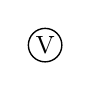
\begin{tikzpicture}[baseline = {([yshift = -3.5pt] current bounding box.center)}]
		\node (V) [circle, draw, scale = 1, inner sep = 1pt, line width = 0.5pt] at (0, 1){\small V};
	\end{tikzpicture}
} % ~{\Large\textcircled{\small V}}~

\newcommand\slidingrheostat{
	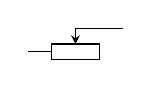
\begin{tikzpicture}[baseline = {([yshift = -3.5pt] current bounding box.center)}]
		\draw (0, 0) rectangle (0.6, 0.2);
		\draw (-0.3, 0.1) -- (0, 0.1);
		\draw [-stealth] (0.3, 0.4) -- (0.3, 0.2);
		\draw [line join = miter] (0.9, 0.4) -- (0.3, 0.4) -- (0.3, 0.3);
	\end{tikzpicture}
}

\newpage
\section{电荷}

\vspace{10pt}
\begin{itemize}
\item 物体能够吸引轻小物体,就说物体带了电,即物体带了\blue{电荷}(electric charge). 带了电荷的物体叫做\blue{带电体}.
\item 使物体带电叫做\blue{起电}. 用摩擦的方式使物体带点叫做\blue{摩擦起电}(electrification by friction).
\item 自然界\blue{只有}两种电荷.
\item 用丝绸摩擦过的玻璃棒带的电荷叫做\blue{正电荷}(positive charge). 用毛皮摩擦过的橡胶棒带的电荷叫做\blue{负电荷}(negative charge).
\item \blue{同种}电荷相互\blue{排斥},\blue{异种}电荷相互\blue{吸引}.
\item 电荷的多少叫做\blue{电荷量}(electric quantity),简称\blue{电量}. 用 \blue{$\bm Q$} 或 \blue{$\bm q$} 表示. 在国际单位制重,电荷量的单位是\blue{库仑}(coulomb),简称\blue{库}. 符号是 \blue{$\bf C$}. 正电荷的电荷量为正值,负电荷的电荷量为负值.
\item \blue{验电器}和\blue{静电计}.
\item 两种电荷互相完全抵消叫做\blue{中和}.
\item 物质是由\blue{分子}构成的,分子是由\blue{原子}构成的.
\item 原子是由带正电的\blue{原子核}和带负电的\blue{电子}(electron)组成的.
\item 原子核是由带正电的\blue{质子}和不带电的\blue{中子}组成的.
\item 每个原子中质子与电子的\blue{数量相等},质子与电子所带的\blue{电荷量相同}.
\item 摩擦起电的本质事电荷从一个物体\blue{转移}到另一个物体.
\item 金属原子中能脱离原子核的束缚而在金属中自由运动的电子叫做\blue{自由电子}(free electron).
\item 失去自由电子的原子叫做\blue{离子}(ion).
\item 质子、电子所带的电荷量(\blue{最小的电荷量})叫做\blue{元电荷}(elementary charge),用 \blue{$\bm e$} 表示. 有:
\mathline{e\approx1.6\times10^{-19}\text{C}}
\item 所有带电体的电荷量都是 $e$ 的整数倍,不是连续变化的,即量子化的.
\item 电子的电荷量 $e$ 与质量 $m_e$ 之比叫做\blue{电子的比荷}(specific charge). 电子的质量 $m_e=9.11\times10^{-31}\text{kg}$,则电子的比荷为:
$$
e:m_e\approx1.76\times10^{11}\text{C}/\text{kg}
$$
\end{itemize}
\newpage
\section{电路}

\subsection{简单电路}
\vspace{10pt}
\begin{itemize}
\item \blue{电路}(electric circuit),即用导线将用电器、电源、开关连接起来.
\item \blue{电源}(power supply),即提供电能的装置,如电池、发电机.
\item \blue{用电器},即消耗电能的装置,如灯泡、电动机.
\item \blue{开关},即控制电路通断的装置,如单刀单掷开关、单刀双掷开关.
\item \blue{导线}通常由绝缘外皮和金属内芯(铜或铝)组成.
\item 处处连通的电路叫做\blue{通路}(\blue{闭合电路}). 某处断开的电路叫做\blue{断路}(\blue{开路}).
\item \blue{直接}用导线将电源的正、负极连接起来的电路叫做\blue{短路}.
\item 闭合电路中,用电器两端被导线直接连通叫做用电器被\blue{短接}.
\item 用符号表示电路连接的图叫做\blue{电路图}.
\item \blue{串联}(series connection)和\blue{并联}(parallel connection).
\item \blue{串联电路}和\blue{并联电路}.
\item 串联电路中各用电器相互影响,并联电路各用电器互不影响.
\end{itemize}
\section{欧姆定律}

\subsection{电流与电压、电阻的关系}
\begin{itemize}
\item 在\blue{电阻一定}时,通过导体的电流与导体两端的电压成正比.
\item 在\blue{电压一定}时,通过导体的电流与导体的电阻成正比.
\item \blue{欧姆定律}(Ohm's law),即导体中的电流,跟导体两端的电压成正比,跟导体的电阻成反比. 有:
\mathline{I=\frac UR}
\newline 欧姆定律对金属、电解液适用,对半导体、电离气体不适用.
\end{itemize}

\subsection{电阻的测量}
\begin{itemize}
\item 伏安法测电阻,即利用 $R=\frac UI$ 测量电阻.
\item 小灯泡是非线性元件,其伏安特性曲线如图.
\begin{figure}[H]
	\centering
	\begin{tikzpicture}
	\begin{axis}[
		axis lines = middle,
		xmin = 0, xmax = 10,
		ymin = 0, ymax = 10,
		smooth, thick,
		xlabel = {$U/\text{V}$}, ylabel = {$I/\text{A}$},
		xlabel style = {anchor = north},
		ylabel style = {anchor = east},
		xtick = \empty,	ytick = \empty,
		samples = 200,
	]
		\addplot+[no marks, domain = 0 : 10]{log10(x + 1) / log10(1.35)};
	\end{axis}
	\node at (0, 0) [below = 5pt, left = -2pt] {$O$};
	\end{tikzpicture}
	\titlename{小灯泡的伏安特性曲线}
\end{figure}
\end{itemize}

\subsection{串、并联电路中的分压、分流规律}
\begin{itemize}
\item 串联分压,即 \blue{$\bm{U_1:U_2:\cdots:U_n=R_1:R_2:\cdots:R_n}$}.
\item 并联分流,即 \blue{$\bm{I_1:I_2:\cdots:I_n=\frac1{R_1}:\frac1{R_2}:\cdots:\frac1{R_n}}$}.
\end{itemize}

\subsection{串、并联电路中电阻的关系}
\begin{itemize}
\item 若电阻 $R$ 产生的效果与两个电阻 $R_1$ 和 $R_2$ 产生的效果相同,则电阻 $R$ 叫做 $R_1$ 和 $R_2$ 的\blue{等效电阻}.
\item 在串联电路中,有 \blue{$\bm{R=R_1+R_2+\cdots+R_n}$},即\blue{串联电路中,等效电阻等于各串联电阻之和}.
\item 在并联电路中,有 \blue{$\bm{\frac1R=\frac1{R_1}+\frac1{R_2}+\cdots+\frac1{R_n}}$},即\blue{并联电路中,等效电阻的倒数等于各并联电阻的倒数之和}. 
\item 两个电阻 $R_1$ 和 $R_2$ 串联时,其等效电阻 \blue{$\bm{R=\frac{R_1R_2}{R_1+R_2}}$}.
\end{itemize}
\section{电功和电功率}

\subsection{电功和电能}
\begin{itemize}
\item \blue{电能}(electric energy)可以转化为其他形式的能. 单位是\blue{焦耳},简称\blue{焦},符号是 \blue{$\bf J$}. 常用单位还有\blue{千瓦时},简称\blue{度},符号是 \blue{$\bf kW\cdot h$}. 换算关系是 \blue{$\bf 1kW\cdot h=3.6\times10^6J$}.
\item 电流做的功叫做\blue{电功}(electric work). 用 \blue{$\bm W$} 表示. 单位是\blue{焦耳},简称\blue{焦},符号是 \blue{$\bf J$}.
\item 电流做了多少功,就有多少电能转化为其他形式的能.
\item 电功等于电压 $U$、电流 $I$ 和通电时间 $t$ 的乘积,即:
\mathline{W=UIt}
\item 根据 $U=IR$,电流通过电阻 $R$ 做的功为:
$$
W=I^2Rt~~或~~W=\frac{U^2}Rt
$$
\item 电功或电能的计量仪器叫做\blue{电能表}(电度表).
\end{itemize}

\subsection{电功率}
\begin{itemize}
\item \blue{电功率}(electric power)是表示\blue{电能做功快慢}的物理量. 用 \blue{$\bm P$} 表示. 单位是\blue{瓦特},简称\blue{瓦},符号是 \blue{$\bf W$}. 常用单位还有千瓦(\blue{$\bf kW$})、毫瓦(\blue{$\bf mW$}). 换算关系是 \blue{$\bf1kW=10^3W$},\blue{$\bf1mW=10^{-3}W$}.
\item 电功率等于电流 $U$ 和电压 $I$ 的乘积,即:
\mathline{P=\frac Wt=UI}
\item 根据 $U=IR$,电流通过电阻 $R$ 的电功率为:
$$
P=I^2R~~或~~P=\frac{U^2}R
$$
\item 用电器正常工作时的电压叫做\blue{额定电压}(rated voltage),用电器在额定电压下工作时的电功率叫做\blue{额定功率}(rated power).
\end{itemize}

\subsection{焦耳定律}
\begin{itemize}
\item 电流通过导体的电能转化为内能,这种现象叫做\blue{电流的热效应}.
\item 电流的效应包括热效应、磁效应和化学效应.
\item \blue{焦耳定律}(Joule's law),即电流通过导体产生的热量 $Q$ 跟电流 $I$ 的二次方成正比,跟导体的电阻 $R$ 成正比,跟通电时间 $t$ 成正比. 即:
\mathline{Q=I^2rt}
\end{itemize}